% Options for packages loaded elsewhere
% Options for packages loaded elsewhere
\PassOptionsToPackage{unicode}{hyperref}
\PassOptionsToPackage{hyphens}{url}
\PassOptionsToPackage{dvipsnames,svgnames,x11names}{xcolor}
%
\documentclass[
  letterpaper,
  DIV=11,
  numbers=noendperiod]{scrartcl}
\usepackage{xcolor}
\usepackage{amsmath,amssymb}
\setcounter{secnumdepth}{5}
\usepackage{iftex}
\ifPDFTeX
  \usepackage[T1]{fontenc}
  \usepackage[utf8]{inputenc}
  \usepackage{textcomp} % provide euro and other symbols
\else % if luatex or xetex
  \usepackage{unicode-math} % this also loads fontspec
  \defaultfontfeatures{Scale=MatchLowercase}
  \defaultfontfeatures[\rmfamily]{Ligatures=TeX,Scale=1}
\fi
\usepackage{lmodern}
\ifPDFTeX\else
  % xetex/luatex font selection
\fi
% Use upquote if available, for straight quotes in verbatim environments
\IfFileExists{upquote.sty}{\usepackage{upquote}}{}
\IfFileExists{microtype.sty}{% use microtype if available
  \usepackage[]{microtype}
  \UseMicrotypeSet[protrusion]{basicmath} % disable protrusion for tt fonts
}{}
\makeatletter
\@ifundefined{KOMAClassName}{% if non-KOMA class
  \IfFileExists{parskip.sty}{%
    \usepackage{parskip}
  }{% else
    \setlength{\parindent}{0pt}
    \setlength{\parskip}{6pt plus 2pt minus 1pt}}
}{% if KOMA class
  \KOMAoptions{parskip=half}}
\makeatother
% Make \paragraph and \subparagraph free-standing
\makeatletter
\ifx\paragraph\undefined\else
  \let\oldparagraph\paragraph
  \renewcommand{\paragraph}{
    \@ifstar
      \xxxParagraphStar
      \xxxParagraphNoStar
  }
  \newcommand{\xxxParagraphStar}[1]{\oldparagraph*{#1}\mbox{}}
  \newcommand{\xxxParagraphNoStar}[1]{\oldparagraph{#1}\mbox{}}
\fi
\ifx\subparagraph\undefined\else
  \let\oldsubparagraph\subparagraph
  \renewcommand{\subparagraph}{
    \@ifstar
      \xxxSubParagraphStar
      \xxxSubParagraphNoStar
  }
  \newcommand{\xxxSubParagraphStar}[1]{\oldsubparagraph*{#1}\mbox{}}
  \newcommand{\xxxSubParagraphNoStar}[1]{\oldsubparagraph{#1}\mbox{}}
\fi
\makeatother


\usepackage{longtable,booktabs,array}
\newcounter{none} % for unnumbered tables
\usepackage{calc} % for calculating minipage widths
% Correct order of tables after \paragraph or \subparagraph
\usepackage{etoolbox}
\makeatletter
\patchcmd\longtable{\par}{\if@noskipsec\mbox{}\fi\par}{}{}
\makeatother
% Allow footnotes in longtable head/foot
\IfFileExists{footnotehyper.sty}{\usepackage{footnotehyper}}{\usepackage{footnote}}
\makesavenoteenv{longtable}
\usepackage{graphicx}
\makeatletter
\newsavebox\pandoc@box
\newcommand*\pandocbounded[1]{% scales image to fit in text height/width
  \sbox\pandoc@box{#1}%
  \Gscale@div\@tempa{\textheight}{\dimexpr\ht\pandoc@box+\dp\pandoc@box\relax}%
  \Gscale@div\@tempb{\linewidth}{\wd\pandoc@box}%
  \ifdim\@tempb\p@<\@tempa\p@\let\@tempa\@tempb\fi% select the smaller of both
  \ifdim\@tempa\p@<\p@\scalebox{\@tempa}{\usebox\pandoc@box}%
  \else\usebox{\pandoc@box}%
  \fi%
}
% Set default figure placement to htbp
\def\fps@figure{htbp}
\makeatother





\setlength{\emergencystretch}{3em} % prevent overfull lines

\providecommand{\tightlist}{%
  \setlength{\itemsep}{0pt}\setlength{\parskip}{0pt}}



 


\KOMAoption{captions}{tableheading}
\makeatletter
\@ifpackageloaded{caption}{}{\usepackage{caption}}
\AtBeginDocument{%
\ifdefined\contentsname
  \renewcommand*\contentsname{Table of contents}
\else
  \newcommand\contentsname{Table of contents}
\fi
\ifdefined\listfigurename
  \renewcommand*\listfigurename{List of Figures}
\else
  \newcommand\listfigurename{List of Figures}
\fi
\ifdefined\listtablename
  \renewcommand*\listtablename{List of Tables}
\else
  \newcommand\listtablename{List of Tables}
\fi
\ifdefined\figurename
  \renewcommand*\figurename{Figure}
\else
  \newcommand\figurename{Figure}
\fi
\ifdefined\tablename
  \renewcommand*\tablename{Table}
\else
  \newcommand\tablename{Table}
\fi
}
\@ifpackageloaded{float}{}{\usepackage{float}}
\floatstyle{ruled}
\@ifundefined{c@chapter}{\newfloat{codelisting}{h}{lop}}{\newfloat{codelisting}{h}{lop}[chapter]}
\floatname{codelisting}{Listing}
\newcommand*\listoflistings{\listof{codelisting}{List of Listings}}
\makeatother
\makeatletter
\makeatother
\makeatletter
\@ifpackageloaded{caption}{}{\usepackage{caption}}
\@ifpackageloaded{subcaption}{}{\usepackage{subcaption}}
\makeatother
\usepackage{bookmark}
\IfFileExists{xurl.sty}{\usepackage{xurl}}{} % add URL line breaks if available
\urlstyle{same}
% fallback for those not using the hyperref driver hyperxmp:
\makeatletter
\@ifundefined{xmpquote}{\newcommand{\xmpquote}[1]{#1}}{}
\makeatother
\hypersetup{
  pdftitle={Tool Radius Compensation},
  pdfauthor={Paolo Bosetti},
  colorlinks=true,
  linkcolor={blue},
  filecolor={Maroon},
  citecolor={Blue},
  urlcolor={Blue},
  pdfcreator={LaTeX via pandoc}}


\title{Tool Radius Compensation}
\usepackage{etoolbox}
\makeatletter
\providecommand{\subtitle}[1]{% add subtitle to \maketitle
  \apptocmd{\@title}{\par {\large #1 \par}}{}{}
}
\makeatother
\subtitle{Digital Manufacturing\\

\includegraphics[width=\linewidth,height=0.3125in,keepaspectratio]{images/by-nc-sa.png}}
\author{Paolo Bosetti}
\date{\emph{Updated:} 14/10/2026}
\begin{document}
\maketitle

\renewcommand*\contentsname{Table of contents}
{
\setcounter{tocdepth}{3}
\tableofcontents
}

\section{Tool radius compensation
(TRC)}\label{tool-radius-compensation-trc}

A possible feature to implement for the personal project

\subsection{TRC and G-code}\label{trc-and-g-code}

\begin{itemize}
\tightlist
\item
  G-code standard supports a feature for offsetting the tool trajectory
  to the left or to the right of the trajectory by an amount equal to
  the tool radius
\item
  This is only affecting the X-Y projection of the trajectory, Z values
  remain unchanged
\item
  The TRC is set to the left with \texttt{G41}, to the right with
  \texttt{G42} and is disabled with \texttt{G40}
\item
  TRC is fully active at the end of the current block
\end{itemize}

\subsection{Tool radius compensation}\label{tool-radius-compensation}

\begin{itemize}
\tightlist
\item
  TRC offsets the tool center path (programmed points) according to
  \texttt{G41}/\texttt{G42}
\item
  New target points are calculated for each block on the basis of the
  offset intersection with the next block (arc or line)
\item
  Disabled for rapid motions
\end{itemize}

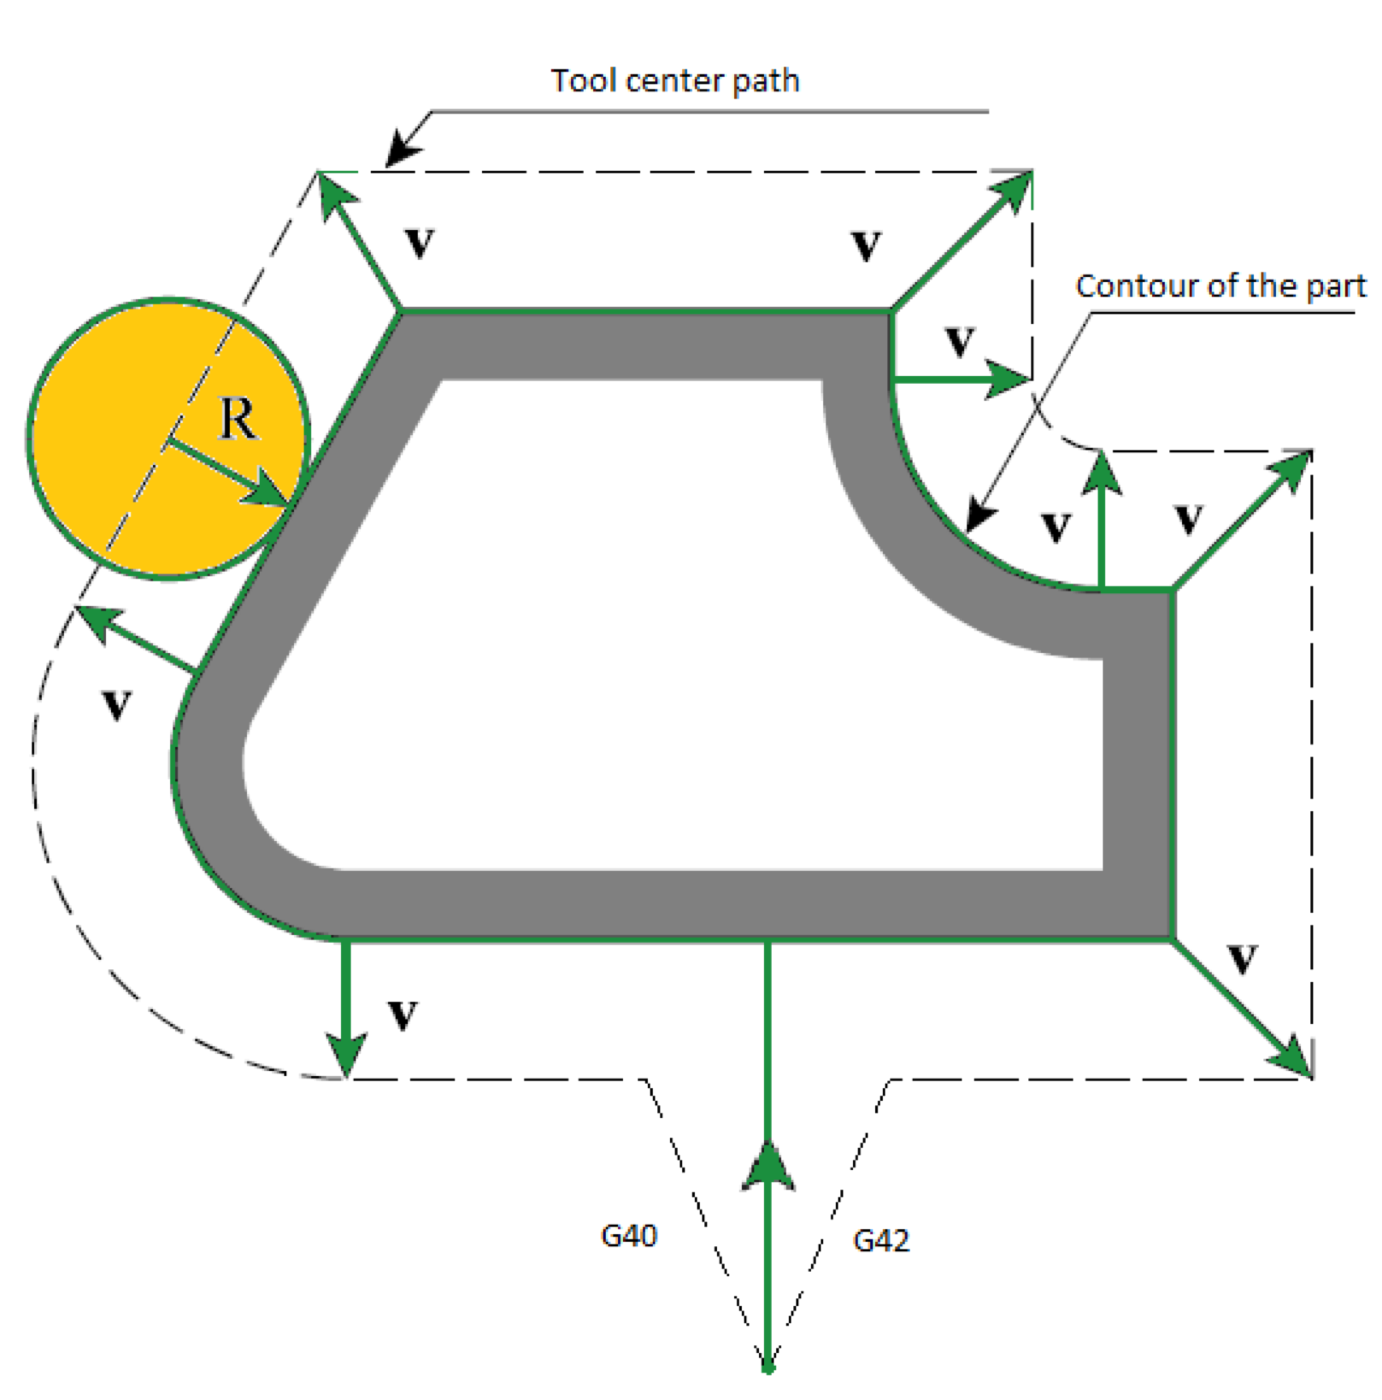
\includegraphics[width=\linewidth,height=4.79167in,keepaspectratio]{images/trc-offset.png}

\subsection{Tool radius compensation:
Line-Line}\label{tool-radius-compensation-line-line}

\subsection{Tool radius compensation:
Line-Circle}\label{tool-radius-compensation-line-circle}

\subsection{Line-Line case}\label{line-line-case}

We need to calculate the point \(D\):

\begin{enumerate}
\def\labelenumi{\arabic{enumi}.}
\tightlist
\item
  Given the line equation \(y = ax + b\), we need to calculate the
  equation of the offset line(s)
\item
  Calculate \(D\) as intercept between the two offset lines
\end{enumerate}

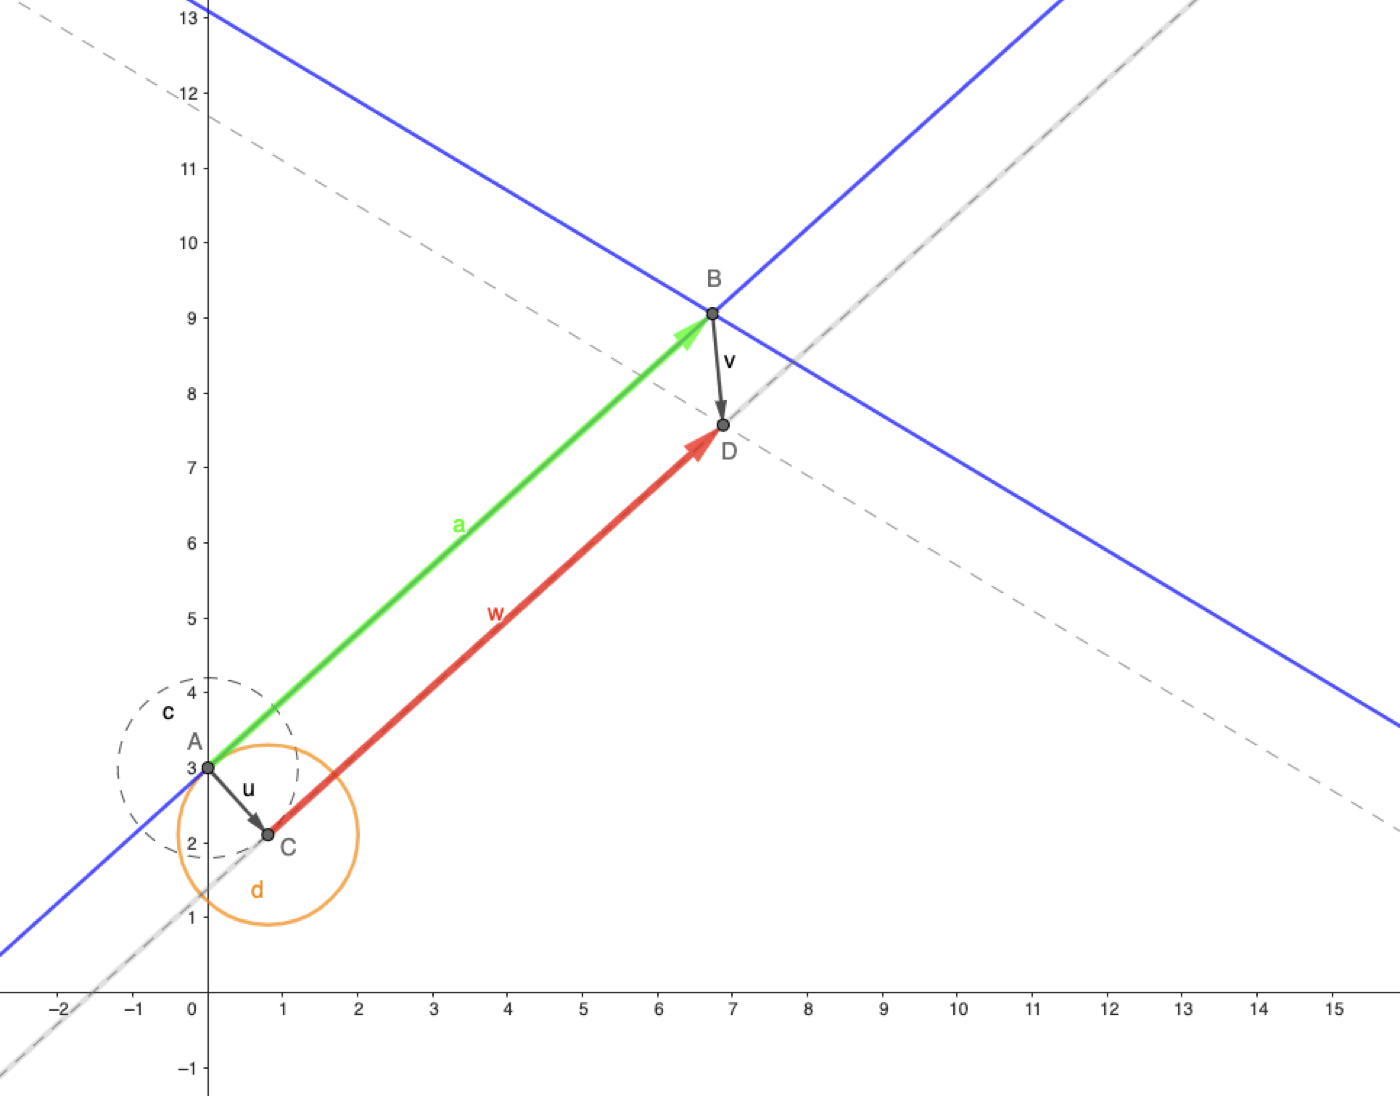
\includegraphics[width=\linewidth,height=4.47917in,keepaspectratio]{images/trc-line-line-1.png}

\subsection{Line-Line case}\label{line-line-case-1}

\begin{itemize}
\tightlist
\item
  Given \(y = ax + b\), the equation of the offset line is
  \(y = ax + b - v\)
\item
  Being \(a = u/r\), it follows that:
  \(v = \sqrt{u^2 + r^2} = r\sqrt{a^2 + 1}\)
\item
  So, \(y = ax + b \pm r\sqrt{a^2 + 1}\)
\item
  \textbf{The sign depends on G41/G42 and on the path direction}
\end{itemize}

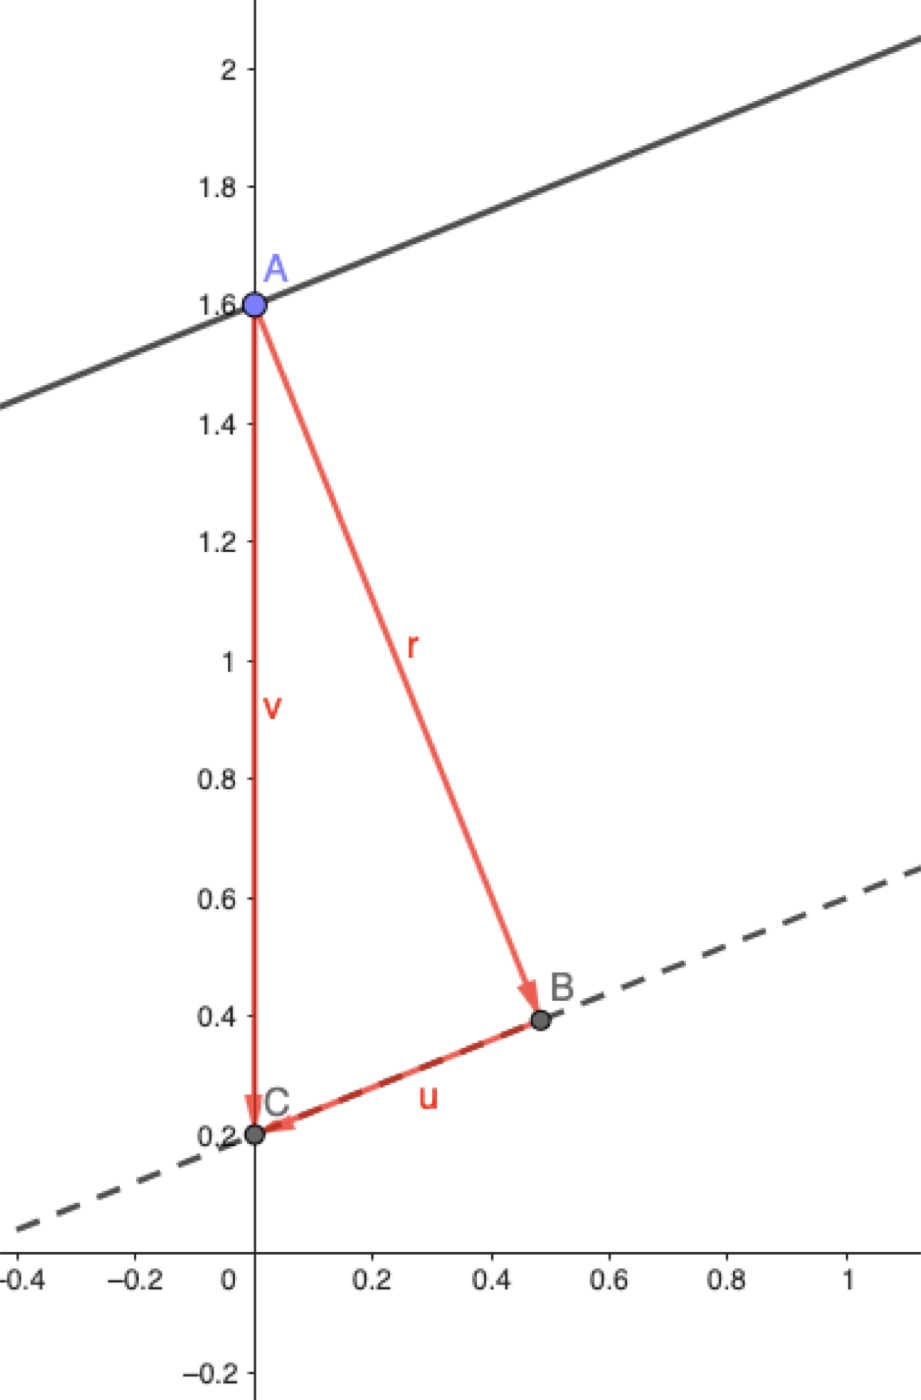
\includegraphics[width=\linewidth,height=4.89583in,keepaspectratio]{images/trc-line-line-2.png}

\subsection{Line-Line case}\label{line-line-case-2}

Intersection \(D\) between

\(y = a_1 x + b_1 - v_1 = a_1 x + b_{o,1}\)

and

\(y = a_2 x + b_2 - v_2 = a_2 x + b_{o,2}\)

has coordinates:

\[(x_i, y_i) = \left(\frac{b_{o,2} - b_{o,1}}{a_1 - a_2}, \frac{b_{o,1}a_2 - b_{o,2}a_1}{a_2 - a_1}\right)\]

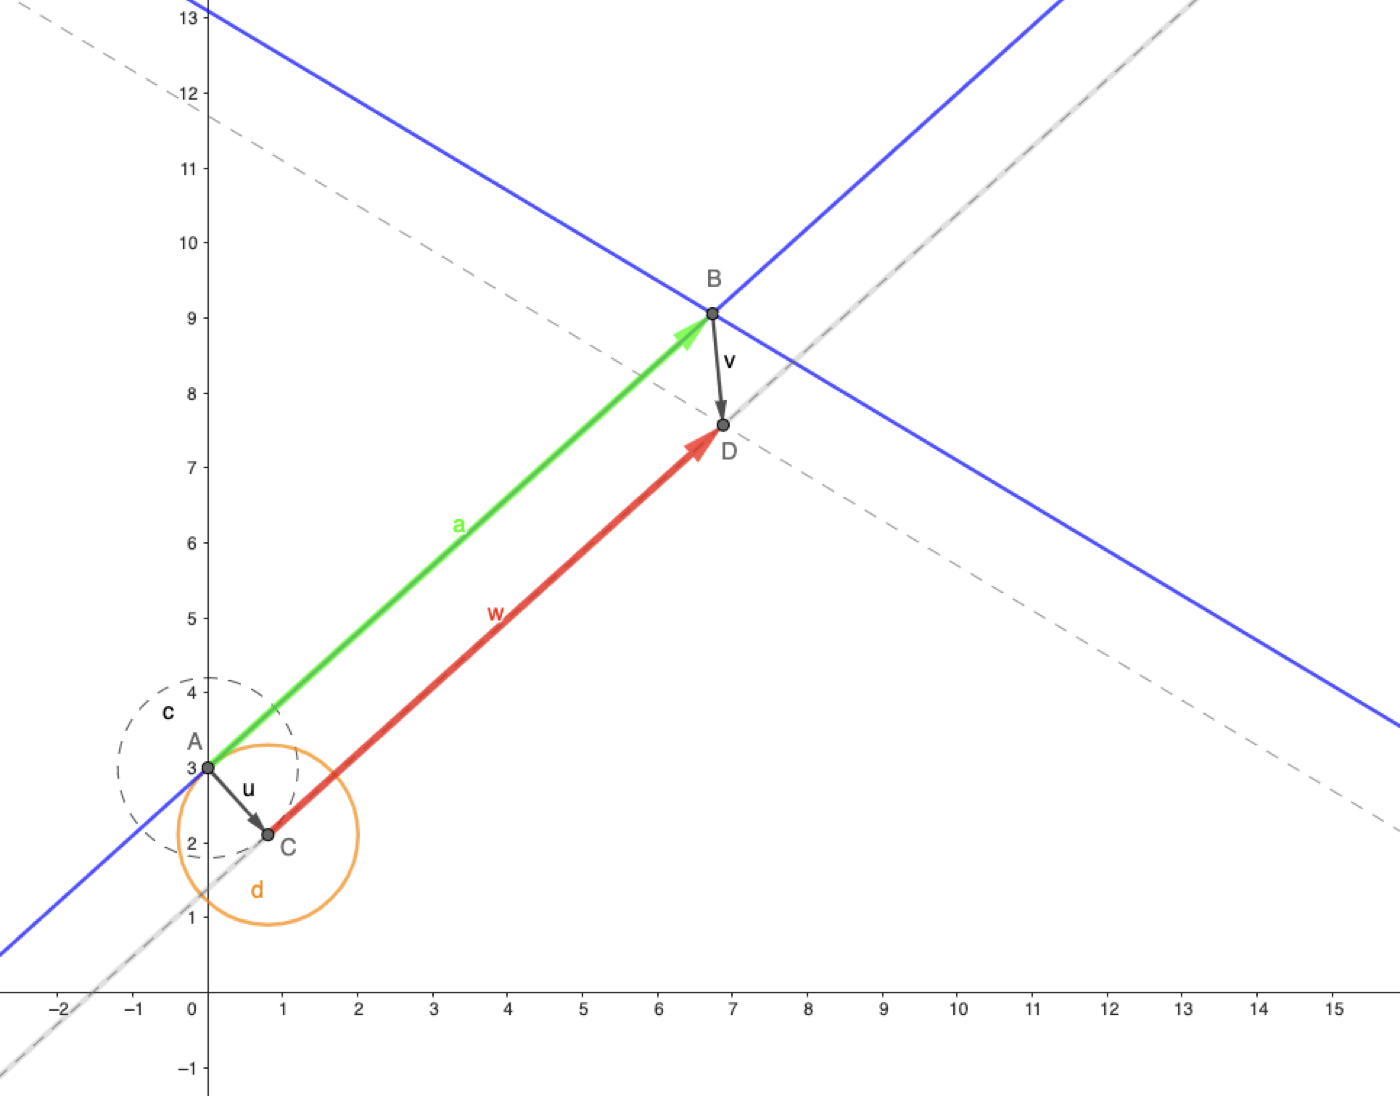
\includegraphics[width=\linewidth,height=4.47917in,keepaspectratio]{images/trc-line-line-1.png}

\subsection{Line-Line case}\label{line-line-case-3}

\begin{itemize}
\tightlist
\item
  \textbf{Exception:} when two segments are collinear
  (\(a = a_1 = a_2\)), the intercept is undefined
\item
  The new intersection node is set at an offset \(r\)
  \textbf{perpendicular} to the segments
\end{itemize}

\[C = \begin{cases} (0, -r), & \text{when } a = 0 \\ r(s, -s/a) \text{ with } s = \frac{a}{|a|}\sqrt{\frac{a^2}{1 + a^2}}, & \text{otherwise} \end{cases}\]

\subsection{Line-Arc (or Arc-Line)}\label{line-arc-or-arc-line}

Similar to line-line case, but with a caveat:

\begin{itemize}
\tightlist
\item
  Line-circle intersection gives two points, \(G\) and \(B_r\): you have
  to select the intersection that is closer to the node to be offset
  (\(B\) in figure)
\end{itemize}

\begin{figure}[H]

{\centering 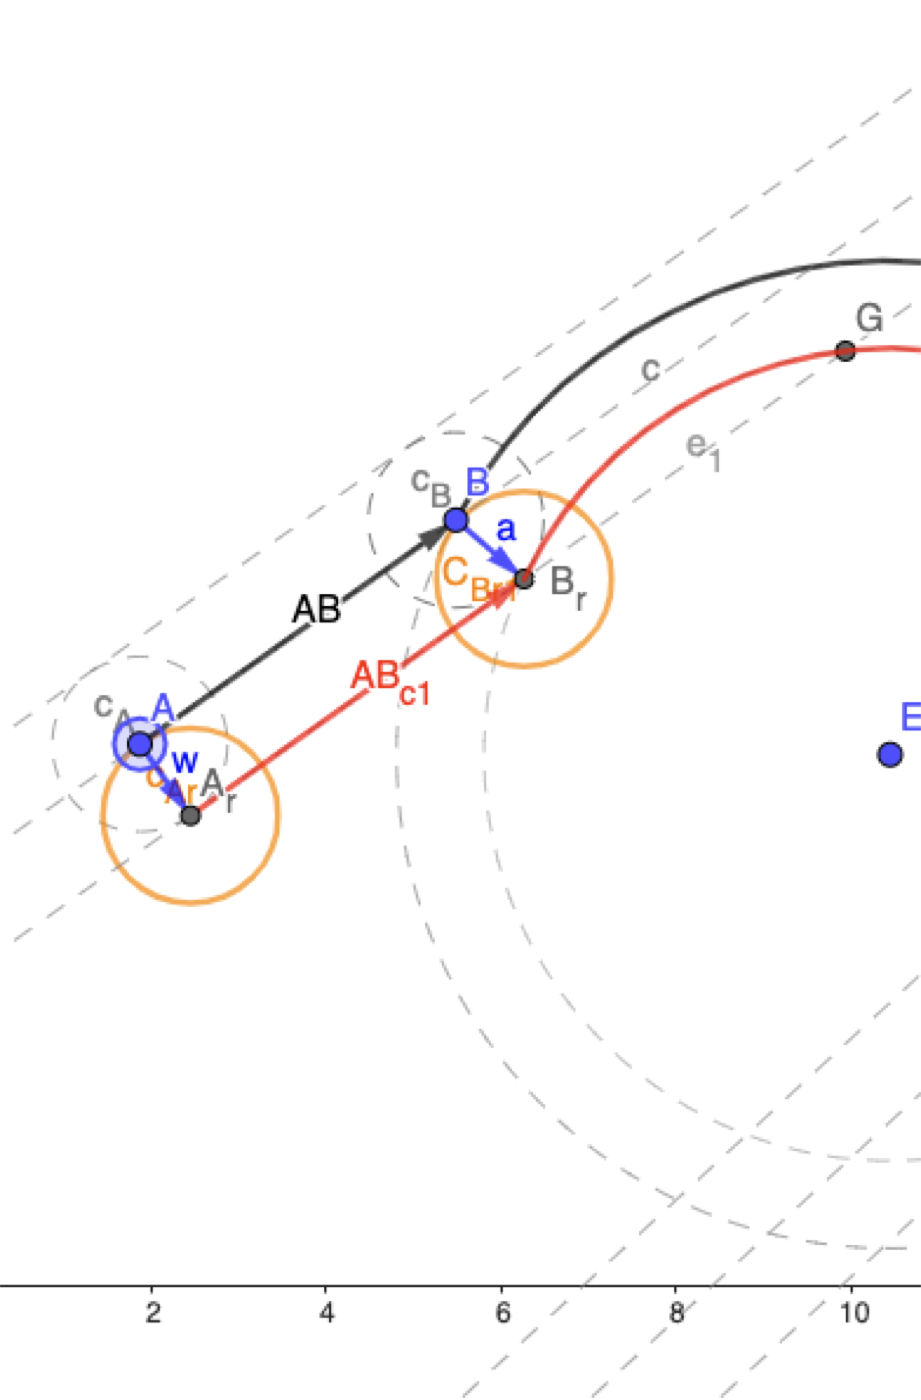
\includegraphics[width=\linewidth,height=4.89583in,keepaspectratio]{images/trc-line-arc-1.png}

}

\caption{Non-tangent line-arc case}

\end{figure}%

\subsection{Line-Arc (or Arc-Line)}\label{line-arc-or-arc-line-1}

Similar to line-line case, but with a caveat:

\begin{itemize}
\tightlist
\item
  Line-circle intersection gives two points, \(G\) and \(B_r\): you have
  to select the intersection that is closer to the node to be offset
  (\(B\) in figure)
\end{itemize}

\begin{figure}[H]

{\centering 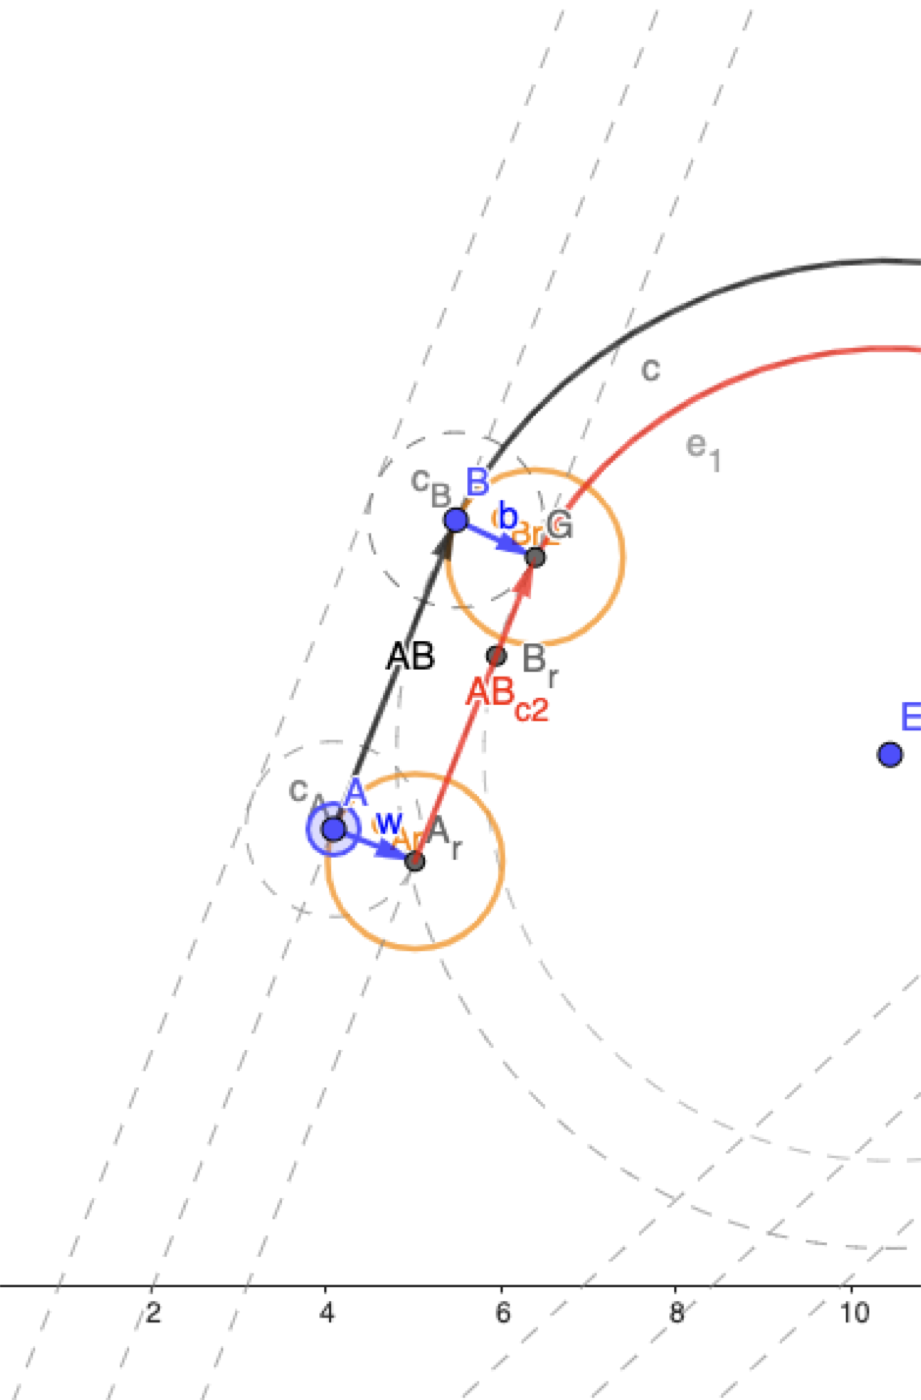
\includegraphics[width=\linewidth,height=4.89583in,keepaspectratio]{images/trc-line-arc-2.png}

}

\caption{Tangent line-arc case}

\end{figure}%

\subsection{Code changes}\label{code-changes}

\textbf{Support for G40/G41/G42}

\begin{itemize}
\tightlist
\item
  An \texttt{enum\ class\ TRCType} with \texttt{NONE}, \texttt{LEFT},
  \texttt{RIGHT}
\item
  An \texttt{TRCType\ \_trc} field in the \texttt{BlockTRC} class
\item
  Proper code in \texttt{BlockTRC::parse()}
\item
  \texttt{\_trc} shall be managed as a \emph{modal} field
  (i.e.~inherited from previous block)
\end{itemize}

\subsection{Code changes}\label{code-changes-1}

\textbf{Support for tool radius}

\begin{itemize}
\tightlist
\item
  The YAML file needs to have a field as:
  \texttt{tools:\ {[}10.0,\ 8.0,\ 5.0,\ 2.5{]}} giving the list of
  available tools and respective radiuses
\item
  The \texttt{Machine} class needs to properly load the tool list into a
  new field: \texttt{vector\textless{}data\_t\textgreater{}\ \_tools}
\item
  Add \texttt{machine::tool\_radius()}, which returns the radius of a
  given tool number
\end{itemize}

\subsection{Code changes}\label{code-changes-2}

\textbf{Support for offset calculation}

\begin{itemize}
\tightlist
\item
  The method \texttt{Block::parse()} needs to change the target of the
  previous block if the previous block has
  \texttt{\_trc\ !=\ TRCType::NONE}
\item
  The target must be changed according to the equations shown above and
  the radius of the current tool
\end{itemize}

\subsection{Code changes}\label{code-changes-3}

\textbf{Support for offset calculation}

\begin{itemize}
\tightlist
\item
  Equations for intersections possibly require:

  \begin{itemize}
  \tightlist
  \item
    \texttt{Block::angle\_with\_prev()}: angle in radians with previous
    block
  \item
    \texttt{Block::equation()}: returns \(a\) and \(b\) as output
    parameters (refs); for an arc, parameters of the implicit equation
    \((x - x_c)^2 + (y - y_c)^2 = r^2\) are available already
  \end{itemize}
\item
  These functions can be private
\end{itemize}

\subsection{Advanced TRC}\label{advanced-trc}

\subsection{Rules}\label{rules}

\begin{itemize}
\tightlist
\item
  You must work alone (I'll check and compare results!)
\item
  Document progress with commits published on GitHub (\textbf{private}
  repo shared with me)
\item
  No help from my side, except these slides
\item
  When you are done, you must discuss your work with me

  \begin{itemize}
  \tightlist
  \item
    If it works (no warnings, errors/errors, works as expected) and it
    is not copied, you get 30/30
  \end{itemize}
\item
  If you implement advanced TRC or impress me with some other clever
  addition, you get 30/30 \emph{cum laude}
\item
  Must be done before the end of next year
\end{itemize}




\end{document}
